
\section{Future Experiments}

\textcolor{red}{There are a large variety of future experiments at the intensity frontier starting or planning in the coming years. Here we have divided them into two categories:  flavour physics experiments which can indirectly probe high energy scales through precision measurements and experiments searching directly for physics beyond the Standard Model. One of the role of the GDR will be to promote the discussions on  which are the priorities and the complementarities among the different physics topics, and which are the most promising experiments  where the French community should  contribute. The mix of data analysis and preparation of new experiments which will characterizes the coming years will be a unique opportunity to ensure the continuity of the successful French involvement in the intensity frontier field. }



%\textcolor{red}{Le premier tient au fait que la diversification des expériences fait que le domaine concerné par ce GDR correspond toujours à des expériences en cours et d’autres en préparation. Je n’ai pas le détail de tous les projets, mais je note (en m’appuyant sur le cours d’Isabelle à Gif en 2015) quelques dates approximatives des projets cités dans le texte : MEG-II 2016-19, Mu3e >2018-20, Mu2e ~ 2020-23, COMET 2020-21, KOTO 2018-20 et Belle-II ~2018->2023-25. Je connais beaucoup moins les manips de recherche des WISP, mais je lis dans le TDR de SHiP que ça pourrait démarrer au plus tôt en 2025 et je présume que parmi les autres manips citées les calendriers s’étalent largement dans les 10 ans à venir. Par ailleurs nous savons que pour LHCb (NA62 avec) les données Run 2 s’arrêtent fin 2018 et reprendront en ~2021 pour 2-3 ans. 
%C’est bien l’illustration que d’aujourd’hui à ~2023-25 (7-9 ans !) nous aurons un mix prise de données - préparation manip - analyse. Il parait donc extrêmement judicieux d’avoir un forum d’échange et de concertation pour bien valoriser les différentes contributions et faciliter les transferts d’expertise et de manpower (un peu oser peut-être) entre ces projets.}



\subsection{Future experimental programs related to $CP$ violation, rare decays of heavy flavours and lepton flavour violating processes}   

As far as $CP$ violation and rare $b$-flavoured hadrons or $\tau$ decays are concerned, the two main players at the horizon of 2025 are the  upgraded LHCb experiment at CERN and the Belle II experiment at KEK.  The synergy and complementarity between the two projects has been assessed clearly in the past and we should ensure within the GDR to follow the progress in both the collaborations. In this respect, we can profit of the connexions established already by members of the GDR with the KEK collegues in the framework of the TYL/FJPPL (Franco-Japan Particle Physics Laboratory) \textcolor{red}{and with the participation into the Belle II-Theory Interface Platform" (B2TIP: https://confluence.desy.de/display/BI/B2TiP+WebHome), a joint theory-experiment effort to study the potential impacts of the Belle II program.}

Several large or medium scale projects related to Flavour Physics are envisaged to probe Beyond Standard Model Physics. Among them, there are prospective studies to educate the possibility to run the LHCb spectrometer in the High Luminosity phase of the LHC or to make use of high intensity beam lines ({\it e.g.} SPS and FCC injectors)  with fixed target experiments.            

A possible long-term strategy for high-energy physics at colliders, after the exploitation of the LHC and its High Luminosity upgrade, considers a tunnel of about 100 km circumference, which takes advantage of the present CERN accelerator complex. The Future Circular Collider (FCC) concept follows on the successful experience and outcomes of the LEP-LHC complex of experiments. A possible first step of the project is to fit in the tunnel a high-luminosity $e^+e^-$ collider aimed at studying comprehensively the electroweak scale with centre-of-mass energies ranging from the $Z$ pole up to beyond the $t \bar t$ production threshold. A  100 TeV proton proton collider is considered as the ultimate goal of the project.  
Future Circular Collider study groups have been formed in a design study hosted by CERN, aiming at a Conceptual Design Report and a review cost in time for next European Strategy milestone (2018-2019). The unprecedented statistics at the $Z$ pole (${\cal O}(10^{12-13} Z$ decays) potentially delivered by the high-luminosity $e^+e^-$ collider can be studied in particular to explore further the Flavour Physics case at large.  

In that framework, several French teams, gathering small groups of experimentalists and phenomenologists, are contributing to the design study in Flavour studies.  
There is a Physics potential of the measurements of rare decays of $b$-hadrons, which can complement  the anticipated results from the current and foreseen $b$-Physics programs (LHCb upgrade and SuperKEKB $B$-factory). In that respect, French contributions are mainly focused on rare electroweak penguins which are likely unique to the FCC: $B^0 \to K^*(892) \tau^+\tau^-$ and $B_s \to \tau^+ \tau^-$.   
The large statistics at the $Z$ pole can be used as well to scrutinize in particular Lepton Flavour Violating (LFV) $Z$ decays, which would serve as an indisputable evidence for New Physics if seen. Heavy right-handed neutrals are natural candidates to explain LFV phenomena. They can be as well searched for directly at FCC-$ee$. A number of low energy experiment are addressing this very question through the search for LFV by muon capture on nuclei ({\it e.g.} COMET in Japan \textcolor{red}{and Mu2e at FNAL}) or the radiative decay of large ensemble of muons ({\it e.g.} MEG \textcolor{red}{and Mu3e at PSI}). 

One objective of the GDR is to address the complementarity of these high intensity machines,  at large scale apparatus or low-energy experiments.  \textcolor{red}{Discussions inside the GDR will also help to identify the emerging technologies and those already mastered at IN2P3 which could play an important role for future experiments, helping the French groups to propose key contributions.} 

\subsection{Weakly interacting new light particles searches}

In this subsection we focus on searches for weakly interacting new light particles, commonly called WISPs, of which the two canonical candidates are hidden photons and axion-like particles. Experiments to search for these are in many cases inexpensive, and can often recycle older experiments. 


The best motivated WISP is the QCD axion itself, which is expected to solve the strong CP problem but is associated with new physics above $10^9$ GeV. Its mass may lie anywhere in the sub-eV range, and it is a very well-motivated dark matter candidate. 


Axion-like particles (ALPs) are (pseudo)-scalars, perhaps cousins of the QCD axion but which do not obtain their masses from QCD. They are characterised by their coupling to photons in a Lagrangian term $\mathcal{L} \supset - \frac{1}{4} g_{a\gamma \gamma} a F_{\mu \nu} \tilde{F}^{\mu \nu}.$ These are highly motivated from top-down constructions as generically arising when symmetries are broken at high scales, and also make attractive dark matter candidates. On the other hand, and perhaps most importantly, there have recently been several studies indicating possible discoveries of such particles in various astronomical observations: either as an explanation for excessive white dwarf cooling or anomalous transparency of the universe to gamma rays, and most excitingly as an explanation for the soft excess of X-rays from the coma cluster (at $200$ eV) and/or the oscillatory modulation of X-rays from the Perseus cluster (and even, perhaps, an explanation for an observed $3.55$ keV X-ray line). These hints all point to a very light ALP ($< 10^{-12}$ eV) with a coupling $g_{a\gamma \gamma} \sim \mathcal{O}(10^{-11} \div 10^{-12}) \mathrm{GeV}^{-1}.$ However, while this is a very interesting region to probe, such a particle could have a wide range of masses and couplings. 
\textcolor{red}{For the motivation of the hidden photon (line 424), maybe it is worth quoting also  the ~7 sigma anomaly in the Be nuclear transition (?).}




Hidden photons are new (massive) gauge bosons which mix kinetically with the visible photon via a dimensionless kinetic-mixing parameter $\chi$. While one motivation of these is as a possible explanation for the $3\sigma$ discrepancy between the measured and calculated value of the muon dipole moment -- this would require a hidden photon in the $\mathcal{O}(100)$ MeV range with $\chi \sim \mathcal{O}(10^{-3})$ -- they also appear generically in top-down constructions of beyond-the-Standard Model physics. They have been proposed as perhaps the most natural force carriers for light dark matter particles, or could even make up the dark matter themselves. Intensity frontier experiments searching for these either search for the particles as dark matter or attempt to directly produce them. In the dark matter case, the assumption that there is a large abundance of particles all around us greatly enhances the reach; on the other hand, for the very light ALPs this is unlikely to be the case. The dark matter searches consist of resonant cavities, helioscopes, and now many more exotic suggestions. Direct searches are broadly photon regeneration experiments (light shining through a wall), electron colliders or beam dumps. \textcolor{red}{Flavour experiments like BaBar, Belle, KLOE and NA48 have been searching for and putting limits on hidden photons, and the flavor experiments effort will continue in the future also within LHCb and Belle II. Other important } upcoming experiments include:
\begin{itemize}
\item Axion haloscopes (magnetic resonant cavity experiments) ADMX-HF, YMCE and WISPDMX at the University of Washington, Yale and Hamburg respectively are all expected to report results soon, probing axion masses in the $\mu$eV range. 
\item The FUNK experiment in Karlsruhe uses a dish antenna to search for dark matter hidden photons.
\item The helioscope SHIPS at Hamburg searches for hidden photons produced in the sun.
\item The REAPR and ALPS-II photon regeneration experiments at Fermilab and DESY respectively will attempt to directly produce ALPs or hidden photons in the lab.
\item The IAXO helioscope at CERN uses a magnetic field to search for ALPs produced in the sun. It is expected to operate over the next decade and there are significant synergies with the French community.
\item The SHIP  beam dump experiment using the SPS proton beam at CERN has a substantial input from French theorists and experimentalists.  
\textcolor{red}{It has the potential to search for messengers of New Physics portals (and additional particles) in the MeV-GeV range. Heavy Neutral leptons (neutrino portal), dark photons (vector portal), light scalars (scalar portal) and pseudoscalars (ALP) can be searched as well as possible supersymmetric partners (neutralinos, sgoldstinos, axinos, saxions...).  The SHiP beamline will be a perfect arena to plan experiments to detect the interactions of the above mentioned particles with matter, i.e. an accelerator based direct dark matter search.}
%It has the potential to search for particles in the GeV range, which included heavier ALPs, as well as other candidates such as right-handed neutrinos. Its development will encompass much of the lifetime of the proposed GDR.
\item There will be electron beam-dump experiments HPS, DarkLight and MESA at SLAC, JLab and Mainz respectively, with the latter running in about 2020. These will provide high intensity competition to hidden-photon searches in the $10-1000$ MeV range.
\item The BMV experiment at Toulouse received ANR funding in 2014 to build phase two and complement its 2007 results. It can perform photon regeneration searches; it also included an X-ray regeneration experiment.
\item There is also a proposal to use the Tore Supra tokamak at Cadarache to search for ALPs. This would be particularly interesting to unite with the plasma physics community. 
\end{itemize}




\begin{figure}[!htb]
\begin{center}
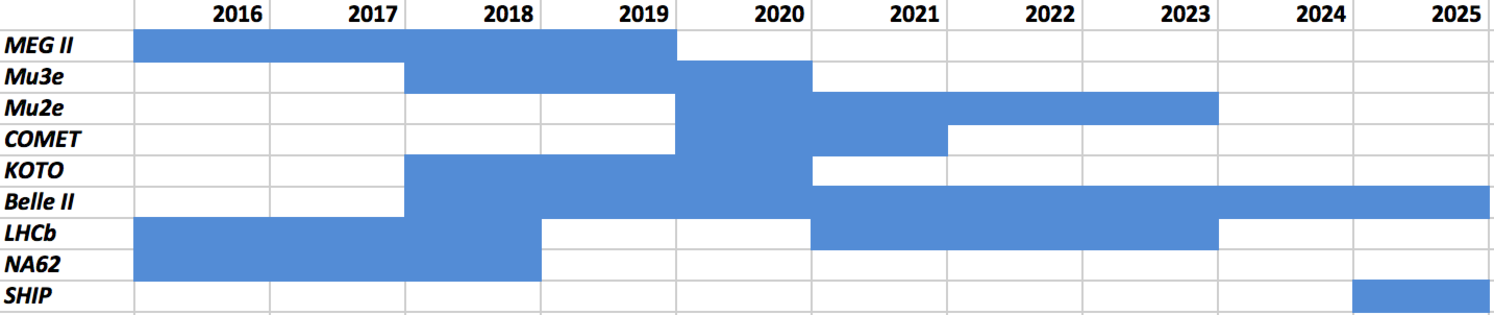
\includegraphics[width=12cm]{timeline.pdf}
\end{center}
\caption{Expected timeline for some of the experiments cited in the text.}%
\label{figphis}%
\end{figure}


